\documentclass[12pt]{beamer}
\usepackage{graphicx}
\usepackage{subcaption}
\usetheme{Madrid} % you can change the theme as per your preference
\title[GPU-Based Simulation]{GPU-Based Simulation and Reinforcement Learning Pipeline for Tracked Ground Robots}
\author{David Korčák}
\date{Prague, January 2025}

\begin{document}

\frame{\titlepage}

% slide 1: Introduction
\section{Introduction}
\begin{frame}{Introduction}
    \begin{itemize}
      \setlength\itemsep{1em}
        \item Original idea: train an RL policy for MARV or TRADR to control their flippers to minimize bouncing, angular speeds etc. 
        \item What actually happened: neither of the simulators were ready to work with flippers and/or were buggy
        \item PyTorch simulator was also quite slow
        \item New objective: develop a PyTorch-based simulator able to handle flipper control, be more numerically stable, bug-free and significantly faster
    \end{itemize}
\end{frame}

% slide 2: Background
\section{Background}
\begin{frame}{Background}
    \begin{itemize}
      \setlength \itemsep{1em}
       \item Why not use an existing simulation engine?
        \item Popular simulation engines like mujoco or brax are optimized for robots with joints and minimal collisions.
        \item No native support for tracked/wheeled robots and complex terrain collisions.
    \end{itemize}
\end{frame}

% slide 4: Simulation Engine
\section{Simulation Engine}
\begin{frame}{Simulation Engine}
  \begin{itemize}
    \item Primarily designed for MARV and TRADR
    \item Simulation based on a pointcloud model of the robot.
    \item Implemented more elaborate and detail-preserving mesh-to-pointcloud conversion.
    \item Interactions modeled using spring-damper systems for terrain forces.
    \item Efficient computation of collision detection and dynamics.
\end{itemize}
\end{frame}

\begin{frame}{Mesh to Pointcloud Conversion}
  \begin{figure}[H]
    \centering
    \includegraphics[width=0.8\textwidth]{fig/full_marv_mesh.png}
    \label{fig:full_marv_mesh}
  \end{figure}
\end{frame}

\begin{frame}{Mesh to Pointcloud Conversion}
  % \vspace{-0.5cm}
  \begin{figure}[H]
    \centering
    % row 1
    \begin{subfigure}[t]{0.25\textwidth}
        \centering
        \includegraphics[width=\textwidth]{fig/full_flipper_mesh.png} % replace with your image path
        \subcaption{Full flipper mesh.}
        \label{fig:fig1}
    \end{subfigure}
    \hspace{1cm}
    \begin{subfigure}[t]{0.25\textwidth}
        \centering
        \includegraphics[width=\textwidth]{fig/flipper_delaunay.png} % replace with your image path
        \subcaption{Delaunay triangulation}
        \label{fig:fig2}
    \end{subfigure}
  
    % row 2
    \begin{subfigure}[t]{0.25\textwidth}
        \centering
        \includegraphics[width=\textwidth]{fig/flipper_surface_points.png} % replace with your image path
        \subcaption{Extracted surface points.}
        \label{fig:fig3}
    \end{subfigure}
    \hspace{1cm}
    \begin{subfigure}[t]{0.25\textwidth}
        \centering
        \includegraphics[width=\textwidth]{fig/flipper_clustered.png} % replace with your image paths
        \subcaption{Clustered surface points.}
        \label{fig:fig4}
    \end{subfigure}

  \end{figure}
  
\end{frame}

% slide 5: GPU Optimization
\section{GPU Optimization}
\begin{frame}{GPU Optimization}
    \begin{itemize}
        \item Leveraging PyTorch for gpu-accelerated matrix operations.
        \item Conditional branching removed to avoid GPU thread divergence and halting.
        \item Torch's new compile functionality used for kernel optimization.
    \end{itemize}
\end{frame}

\begin{frame}{Forward Computational Graph}
  \begin{figure}[H]
    \centering
    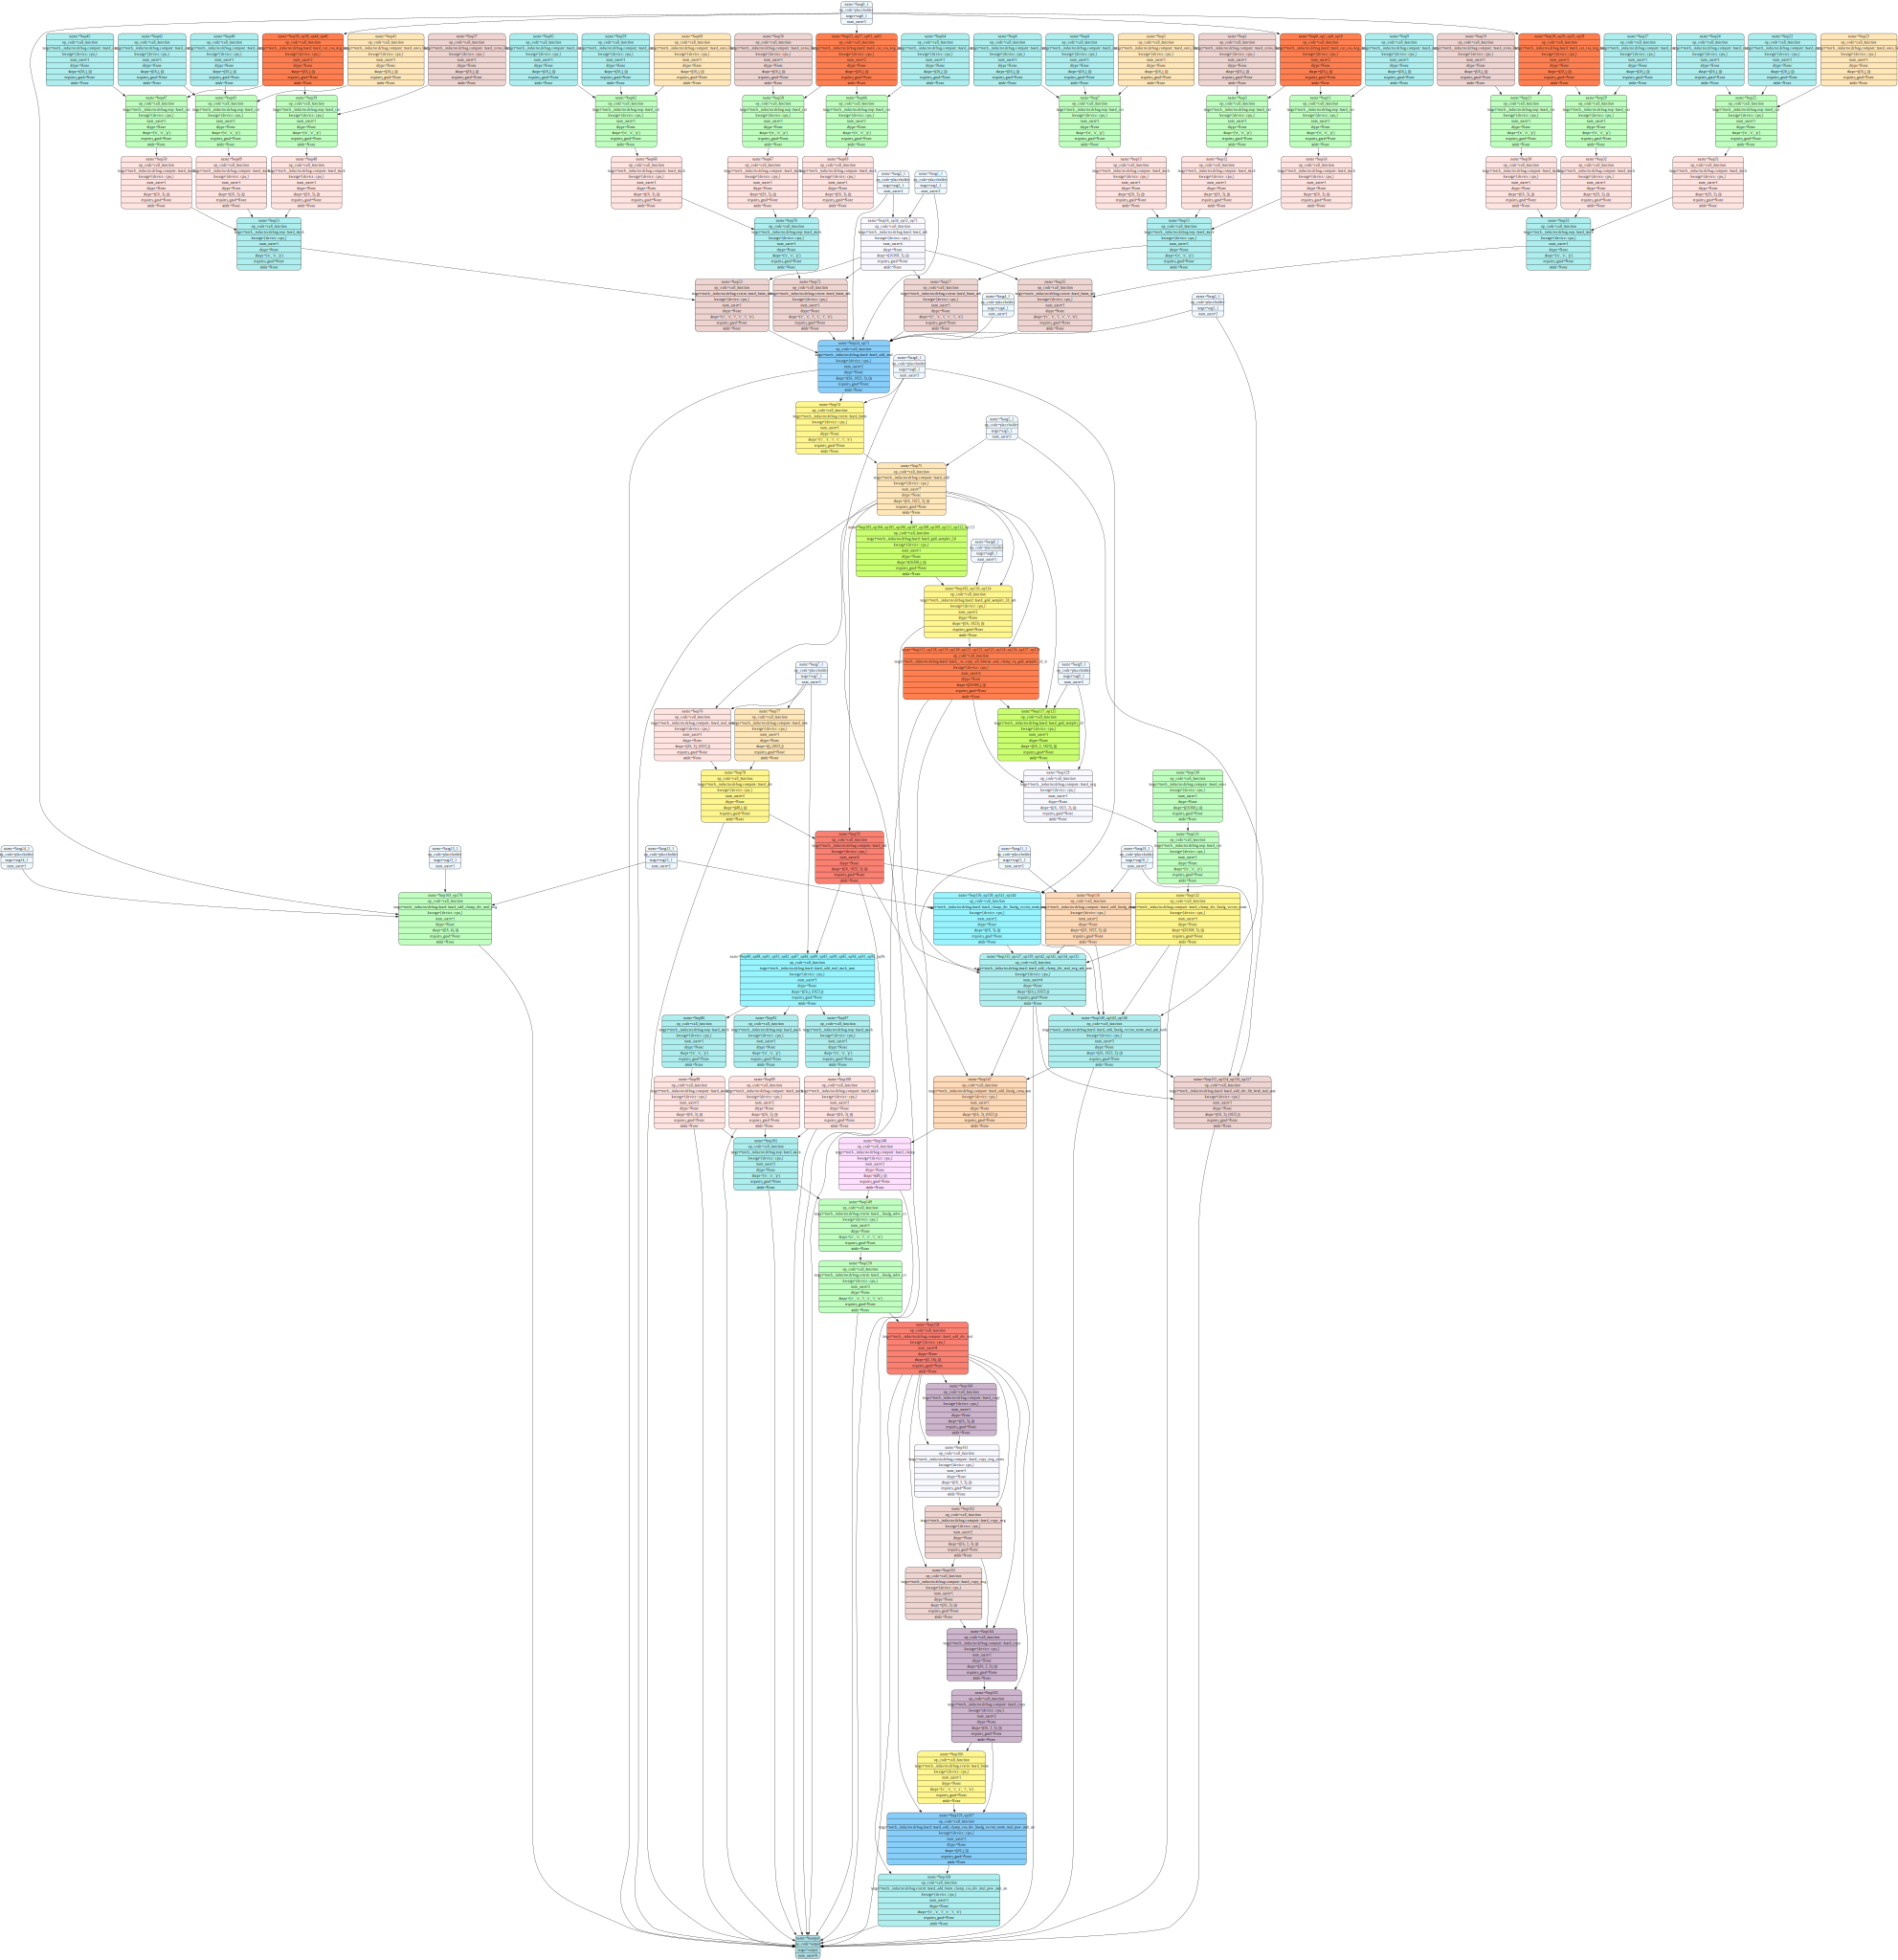
\includegraphics[width=0.6\textwidth]{fig/graph_diagram.pdf}
    \label{fig:speedup}
  \end{figure}
\end{frame}


% slide 6: Performance Evaluation
\section{Performance Evaluation}
\begin{frame}{Performance Evaluation - CPU (M1 Pro)}
  \begin{figure}[H]
    \centering
    \includegraphics[width=0.9\textwidth]{fig/benchmark_cpu_m1.pdf}
    \label{fig:cpu_speedup}
  \end{figure}
\end{frame}

\begin{frame}{Performance Evaluation - GPU (A100)}
  \begin{figure}[H]
    \centering
    \includegraphics[width=0.9\textwidth]{fig/benchmark_cuda_2025-01-12_21-41-37_eager.pdf}
    \label{fig:gpu_speedup}
  \end{figure}
\end{frame}

% slide 7: Reinforcement Learning Environment
\section{RL Environment}
\begin{frame}{Reinforcement Learning Environment}
    \begin{itemize}
        \item Implemented a basic RL framework and environment using TorchRL (native interop with Tensors, devices, datatypes, shapes).
        \item Observation types: bird-view heightmap camera and 3d lidar pointcloud.
        \item Random procedural terrain generation.
    \end{itemize}
\end{frame}

\begin{frame}{Procedural Terrain Generation}
  \centering
  \vspace{-0.2cm}
  \begin{figure}[H]
    \begin{subfigure}[t]{0.6\textwidth}
      \includegraphics[width=0.9\textwidth]{fig/rough_terrain.png}
      \subcaption{Generated terrain with rough preset.}
    \end{subfigure}

    \begin{subfigure}[t]{0.6\textwidth}
      \includegraphics[width=0.9\textwidth]{fig/smooth_terrain.png}
      \subcaption{Generated terrain with smooth preset.}
    \end{subfigure}
  \end{figure}
\end{frame}

% slide 10: Conclusion
\section{Conclusion}
\begin{frame}{Conclusion}
    \begin{itemize}
        \item GPU-friendly simulation engine and basic rl environment developed.
        \item Future work: refine physics models and complete rl experiments.
        \item Merge with Aleš and his more advanced joint modeling
    \end{itemize}
\end{frame}

\end{document}